\subsection{使用 tikz 绘制图形}

\begin{frame}{用 tikz 画了个图}{这部分内容放在了另外一个 tex 文件中}

  代码默认存在 $10$ 台虚拟机,输入状态 $s_t$ 为当前提交任务的类型和 $10$ 台虚拟机的 $T_{idle}$ :
  $$s_t = \left[Type,\, T_{idle}^{(1)},\, T_{idle}^{(2)},\, \dots,\, T_{idle}^{(10)}\right]^T$$

  DQN输出在当前状态 $s_t$ 下,对分配到每台虚拟机的总共 $10$ 个动作的评分。

  \begin{figure}
    \begin{tikzpicture}[scale=0.2,font=\small]
      \draw[->] (-4,0) node[left] {$s_t$} -- (-0.5,0);

      \draw[step=1cm] (0,-4) grid (1,4);
      \node[below] at (0.5,-4) {输入层 $x \in \mathbb{R}^{11}$};

      \draw[->] (1.5,0) -- (16.5,0);
      \node[above right] at (1.5,0) {$ReLU(W_1^Tx+b_1)$};

      \draw[step=1cm] (17,-6) grid (18,6);
      \node[below] at (17.5,-6) {隐藏层 $y \in \mathbb{R}^{20}$};

      \draw[->] (18.5,0) -- (27.5,0);
      \node[above right] at (18.5,0) {$W_2^T y+b_2$};

      \draw[step=1cm] (28,-3) grid (29,3);
      \node[below] at (28.5,-3) {输出层 $q \in \mathbb{R}^{10}$};
    \end{tikzpicture}
  \end{figure}

  其中两层全连接层的参数:$W_1 \in \mathbb{R}^{11 \times 20},\, b_1 \in \mathbb{R}^{20},\, W_2 \in \mathbb{R}^{20 \times 10},\, b_2 \in \mathbb{R}^{10}$ 。
\end{frame}

\subsection{使用 tikz 绘制子图}

\begin{frame}{用 tikz 花了两个子图}

  \begin{figure}
    \centering

    \begin{subfigure}[c]{0.4\textwidth}
      \begin{tikzpicture}
        \draw[->] (0,0) node[below] {$0$} -- (5,0) node[right] {$t$};

        \draw[-] (1,3pt) -- (1,-3pt) node[below] {$W_1$};
        \draw[-] (3.5,3pt) -- (3.5,-3pt) node[below] {$W_2$};

        \node[above] at (2.25,7pt) {$T_2$};
        \draw[<->] (1,5pt) -- (3.5,5pt);

        \node[below=1.5em] at (1,0) {$s$};
        \draw[dashed] (4,0) -- (4,-1.5em) node[below] {$s+t$};
      \end{tikzpicture}

      \caption{$T_2 \leqslant t$}
    \end{subfigure}
    \qquad
    \begin{subfigure}[c]{0.4\textwidth}
      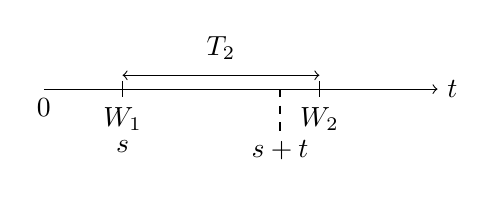
\begin{tikzpicture}
        \draw[->] (0,0) node[below] {$0$} -- (5,0) node[right] {$t$};

        \draw[-] (1,3pt) -- (1,-3pt) node[below] {$W_1$};
        \draw[-] (3.5,3pt) -- (3.5,-3pt) node[below] {$W_2$};

        \node[above] at (2.25,7pt) {$T_2$};
        \draw[<->] (1,5pt) -- (3.5,5pt);

        \node[below=1.5em] at (1,0) {$s$};
        \draw[dashed] (3,0) -- (3,-1.5em) node[below] {$s+t$};
      \end{tikzpicture}

      \caption{$T_2 > t$}
    \end{subfigure}
  \end{figure}

\end{frame}
